\documentclass[11pt]{article}

%% MinionPro fonts 
%\usepackage[lf]{MinionPro}
%\usepackage{MnSymbol}
\usepackage{microtype}

%% Margins
\usepackage{geometry}
\geometry{verbose,letterpaper,tmargin=1in,bmargin=1in,lmargin=1in,rmargin=1in}

%% Other packages
\usepackage{amsmath}
\usepackage{amsthm}
\usepackage[shortlabels]{enumitem}
\usepackage{titlesec}
\usepackage{soul}
\usepackage{tikz}
\usepackage{mathtools}
\usepackage{pgfplots}
\usepackage{tikz-3dplot}
\usepackage{algorithmic}
\usepackage[export]{adjustbox}
\usepackage{tcolorbox}
\usepackage{mathrsfs}
\usepackage{hyperref}

%% Paragraph style settings
\setlength{\parskip}{\medskipamount}
\setlength{\parindent}{0pt}

%% Change itemize bullets
\renewcommand{\labelitemi}{$\bullet$}
\renewcommand{\labelitemii}{$\circ$}
\renewcommand{\labelitemiii}{$\diamond$}
\renewcommand{\labelitemiv}{$\cdot$}

%% Colors
\definecolor{rred}{RGB}{204,0,0}
\definecolor{ggreen}{RGB}{0,145,0}
\definecolor{yyellow}{RGB}{255,185,0}
\definecolor{bblue}{rgb}{0.2,0.2,0.7}
\definecolor{ggray}{RGB}{190,190,190}
\definecolor{ppurple}{RGB}{160,32,240}
\definecolor{oorange}{RGB}{255,165,0}

%% Shrink section fonts
\titleformat*{\section}{\normalsize\bf}
\titleformat*{\subsection}{\normalsize\bf}
\titleformat*{\subsubsection}{\normalsize\it}

% %% Compress the spacing around section titles
\titlespacing*{\section}{0pt}{1.5ex}{0.75ex}
\titlespacing*{\subsection}{0pt}{1ex}{0.5ex}
\titlespacing*{\subsubsection}{0pt}{1ex}{0.5ex}

%% amsthm settings
\theoremstyle{definition}
\newtheorem{problem}{Problem}
\newtheorem{example}{Example}
\newtheorem*{theorem}{Theorem}
\newtheorem*{bigthm}{Big Theorem}
\newtheorem*{biggerthm}{Bigger Theorem}
\newtheorem*{bigcor1}{Big Corollary 1}
\newtheorem*{bigcor2}{Big Corollary 2}

%% tikz settings
\usetikzlibrary{calc}
\usetikzlibrary{patterns}
\usetikzlibrary{decorations}
\usepgfplotslibrary{polar}

%% algorithmic setup
\algsetup{linenodelimiter=}
\renewcommand{\algorithmiccomment}[1]{\quad// #1}
\renewcommand{\algorithmicrequire}{\emph{Input:}}
\renewcommand{\algorithmicensure}{\emph{Output:}}

%% Answer box macros
%% \answerbox{alignment}{width}{height}
\newcommand{\answerbox}[3]{%
  \fbox{%
    \begin{minipage}[#1]{#2}
      \hfill\vspace{#3}
    \end{minipage}
  }
}

%% \answerboxfull{alignment}{height}
\newcommand{\answerboxfull}[2]{%
  \answerbox{#1}{6.38in}{#2} 
}

%% \answerboxone{alignment}{height} -- for first-level bullet
\newcommand{\answerboxone}[2]{%
  \answerbox{#1}{6.0in}{#2} 
}

%% \answerboxtwo{alignment}{height} -- for second-level bullet
\newcommand{\answerboxtwo}[2]{%
  \answerbox{#1}{5.8in}{#2}
}

%% special boxes
\newcommand{\wordbox}{\answerbox{c}{1.2in}{.7cm}}
\newcommand{\catbox}{\answerbox{c}{.5in}{.7cm}}
\newcommand{\letterbox}{\answerbox{c}{.7cm}{.7cm}}

%% Miscellaneous macros
\newcommand{\tstack}[1]{\begin{multlined}[t] #1 \end{multlined}}
\newcommand{\cstack}[1]{\begin{multlined}[c] #1 \end{multlined}}
\newcommand{\ccite}[1]{\only<presentation>{{\scriptsize\color{gray} #1}}\only<article>{{\small [#1]}}}
\newcommand{\grad}{\nabla}
\newcommand{\ra}{\ensuremath{\rightarrow}~}
\newcommand{\maximize}{\text{maximize}}
\newcommand{\minimize}{\text{minimize}}
\newcommand{\subjectto}{\text{subject to}}
\newcommand{\trans}{\mathsf{T}}
\newcommand{\bb}{\mathbf{b}}
\newcommand{\bx}{\mathbf{x}}
\newcommand{\bc}{\mathbf{c}}
\newcommand{\bd}{\mathbf{d}}

%% LP format
%    \begin{align*}
%      \maximize \quad & \mathbf{c}^{\trans} \mathbf{x}\\
%      \subjectto \quad & A \mathbf{x} = \mathbf{b}\\
%                       & \mathbf{x} \ge \mathbf{0}
%    \end{align*}


%% Redefine maketitle
\makeatletter
\renewcommand{\maketitle}{
  \noindent SA405 -- AMP \hfill Rader \S 3.4--Page 103 \\

  \begin{center}\Large{\textbf{\@title}}\end{center}
}
\makeatother

%% ----- Begin document ----- %%
\begin{document}
  
\title{Lesson 8:  Combinatorial Models and the Traveling Salesperson Problem}

\maketitle

\section{Combinatorial Models}

Many optimization problems are naturally modeled by a combinatorial structure, such as a \textbf{graph}. For the next few weeks, we will be talking about several combinatorial optimization models.

Combinatorial optimization problems are usually more general than the network problems we've seen before as they operate on a \textbf{graph} instead of a \textbf{network}. Recall that a network is a special type of graph.

For now, we will develop integer programs to model these problems. Integer programming is appropriate for traveling salesperson and vehicle routing problems (they're NP-Complete which means \textbf{really} hard to solve).
%
%What is the difference between an \textbf{algorithm} and a \textbf{heuristic}?
%
%\answerboxfull{c}{2in}
%
%Is the simplex method an algorithm or a heuristic?
%
%\answerboxfull{c}{1in}


\section{Graph Terminology}


Suppose $G = (V,E)$ is an \emph{undirected} graph. (So far we have worked with directed graphs.) Recall that:
	\begin{itemize}
	\item $V$ is the set of vertices or nodes
	\item $E$ is the set of edges
	\end{itemize}

An undirected graph is different in that the edges can now be traversed in both directions. \vspace{1in}

As a result, it's good to be consistent in naming the edges. For example, using our old style of naming, an edge connecting nodes 1 and 2 could be both $x_{1,2}$ and $x_{2,1}$. As a result, we will always name edges from lower index to higher index.

\newpage


\begin{tcolorbox}
Graph $G$ is \textbf{connected} if for \emph{every} pair of vertices $a,~b \in V$, there exists a \textbf{path} of edges in $G$ connecting $a$ and $b$.  
\end{tcolorbox}

Example: \vspace{2in}

\begin{tcolorbox}
A \textbf{cycle} is a closed path of nodes meaning that the first and last node in the path is the same vertex.
\end{tcolorbox}

Example: \vspace{2in}

\begin{tcolorbox}
If $G$ is a connected graph that contains a \textbf{cycle}, then the removal of a single edge from the cycle does not destroy the connectivity of $G$.
\end{tcolorbox}

\begin{enumerate}[resume]
\item Illustrate a cycle and prove the fact that if $G$ has a cycle, removing any edge from the cycle does not make the graph disconnected.
\end{enumerate}

\newpage



\begin{tcolorbox}
A connected graph that contains no cycles is called a \textbf{tree}.  
\end{tcolorbox}
Example: \vspace{3in}

\begin{tcolorbox}
Trees are \textbf{minimally connected}:  if we remove any edge from a tree, the resulting graph is disconnected.
\end{tcolorbox}
\begin{enumerate}[resume]
\item Convince yourself of the previous fact by drawing a tree on 6 vertices.  Are there any edges you can remove from the graph without losing connectivity?
\end{enumerate}

\vfill

\begin{tcolorbox}
Trees are really important in tons of real world problems. For example, every time you make a Google search or use GoogleMaps an algorithm is called where one of the key parts is analyzing a huge tree. These trees are usually found via an algorithm (not math programming); but they are a structure that come up over and over again.
\end{tcolorbox}


\newpage
%%%
\section{Tours and TSP}

\begin{tcolorbox}
A \textbf{tour} is a closed route that visits every location exactly once.

\smallskip
In graph terminology, a \textbf{tour} is a single cycle (collection of edges) that visits each node exactly once. This is also known as a Hamiltonian Cycle or Hamiltonian Circuit.
\end{tcolorbox}

\begin{problem}
For each graph below, does the set of edges represent a tour through the 6 nodes?  If not, explain why not.

\begin{center}
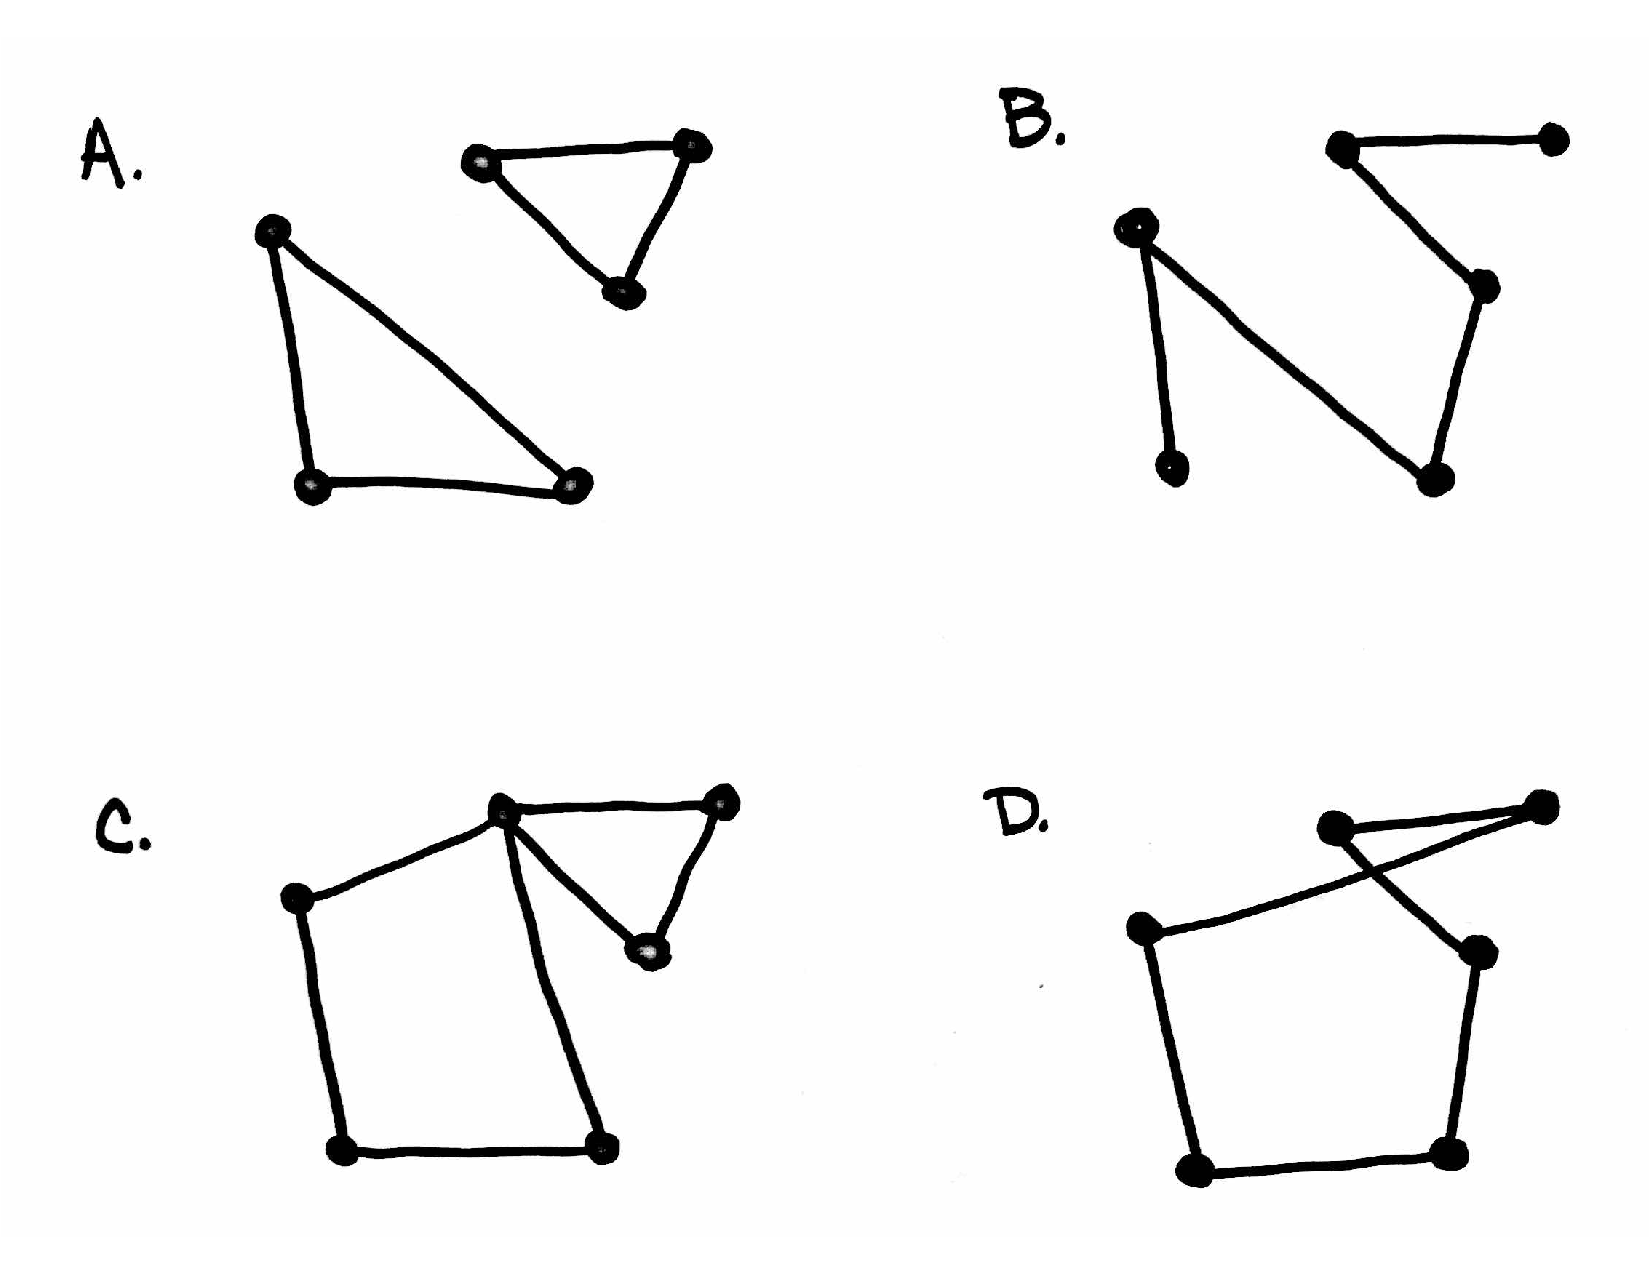
\includegraphics[width=0.6\textwidth]{tours}
\end{center}
\end{problem}

\begin{tcolorbox}
Given a graph $G = (V, E)$ with edge weights (representing costs or distances), the \textbf{Traveling Salesperson Problem (TSP)} seeks a \emph{minimum cost tour of} $G$.
\end{tcolorbox}

\section{History of the TSP}

\begin{itemize}
\item TSP was first studied in the 1930s! The first IP formulation of TSP (which we're studying mostly in these notes) was in 1954.
\item Nowadays TSP has been solved on graphs with as many as 50,000 nodes such as a historic tour of the US.
\url{http://www.math.uwaterloo.ca/tsp/}
\end{itemize}

\newpage

\section{Visiting Graduate Schools: IP Formulation of TSP}

\begin{problem}
A college student is interested in visiting as many graduate schools as possible.
She reasons that a single visit to each school is appropriate, and she wants to 
return to her own campus only after visiting all the schools.  It is conceivable that
she visits the schools in any order, but she would like to minimize the amount of
driving she has to do.  If the distance between schools $i$ and $j$ is $d_{i,j}$ ($i < j$), where the 
matrix $D$ of distances is given below, in which order should she visit the schools?
Note that school 1 is her current school.

\[
D = \left[
\begin{array}{c|ccccc}
& 2 & 3 & 4 & 5 & 6 \\
\hline
1 & 16 & 23 & 14 & 8 & 15 \\
2 & - & 12 & 19 & 9 & 13 \\
3 & - & - & 7 & 25 & 16 \\
4 & - & - & - & 18 & 15 \\
5 & - & - & - & - & 20 \\
\end{array}
\right]
\]

\begin{enumerate}[resume]
\item Draw the graph $G = (V,E)$ of the network below.  Include node labels and edge costs.  Highlight a collection of edges that form a tour of the graph (doesn't have to be the minimum distance tour).

\vfill


\item What type of solution do we want for this problem? What decision (variables) would we make in order to find such a solution? \vfill

\newpage

\item Define the Sets, Variables, and Parameters that are needed for the IP model. 
\vfill 

\item Write the objective function for this model. \vspace{1.25in}

\item There are two types of constraints that should be included in this model:
	\begin{enumerate}
	\item A cycle on $n$ nodes has exactly \catbox edges. Write this constraint in concrete and parameterized form. \vfill
	\item Every node is visited and departed from exactly one time. Thus, each node must be connected to exactly \catbox edges. Write this constraint in both concrete and parameterized form. \vfill
	\end{enumerate}
\end{enumerate}


\newpage
So, at this point, we have a model which given a set of nodes $N$ and edges $E$:
\begin{itemize}
\item Minimizes the total cost of edges selected
\item Enforces that exactly $|N|$ edges are part of the tour
\item Enforces that each node is connected to exactly 2 edges
\end{itemize}

Using the graph of 6 nodes, can you think of a solution that satisfies these constraints but is not a tour? \vfill

\begin{enumerate}[resume]
\item Write a concrete constraint that prevents the graph above from being selected by the solver. \vfill
\item How many constraints of this type would be required to remove all cycles of size 3? \vfill
\end{enumerate}



\begin{tcolorbox}
These type of constraints are called \textbf{cycle-elimination} or often \textbf{subtour-elimination} constraints. As we see above, there are way too many of these to all be included in the model. In practice, these constraints may be added iteratively to eliminate cycles in a solution returned by the solver.  We will do something like this in the context of vehicle routing.
\end{tcolorbox}

\newpage

\section{Subtour Elimination Constraints For More than Three Nodes}

Now, we have seen an example of adding a subtour elimination constraint to eliminate a cycle of size three. Now, suppose our graph has 8 nodes and we obtain the following solution: \vfill


We want to eliminate one of the subtours on four nodes.

\begin{enumerate}[resume]
\item Write a constraint that eliminates this cycle on four nodes from the graph. \vfill
\item What is the drawback of this constraint? \vspace{1in}
\item How can you modify this constraint to address this drawback? \vfill
\item Write this new constraint in parameterized form. \vfill
\end{enumerate}

\newpage

\section{Putting it All Together: Parameterized TSP}

Write the parameterized TSP model.
\end{problem}
\end{document}

